%%=============================================================================
%% Methodologie
%%=============================================================================

\chapter{\IfLanguageName{dutch}{Methodologie}{Methodology}}
\label{ch:methodologie}

%% TODO: Hoe ben je te werk gegaan? Verdeel je onderzoek in grote fasen, en
%% licht in elke fase toe welke stappen je gevolgd hebt. Verantwoord waarom je
%% op deze manier te werk gegaan bent. Je moet kunnen aantonen dat je de best
%% mogelijke manier toegepast hebt om een antwoord te vinden op de
%% onderzoeksvraag.

De methode die werd toegepast om de onderzoeksvraag correct te beantwoorden is het maken van twee proof of concepts en deze te vergelijken en analyseren. Tijdens dit onderzoek wordt in de eerste proof of concept gebruik gemaakt van Azure active directory om een API te gaan beveiligen met bearer authentication. Er wordt ook gekeken naar hoe een client geconfigureerd kan worden om toegang te krijgen tot deze API. Er wordt ook dieper ingegaan op de communicatie tussen de API, de client en Azure active directory. Deze proof of concept is gebaseerd op de client credentials grant type en vergt dus geen input van een gebruiker. In de tweede proof of concept wordt een sign-in met Microsoft gebruikt waardoor hier wel input van de gebruiker verwacht wordt. In deze proof of concept wordt de implicit grant gebruikt. Deze twee methoden worden later vergeleken. Vooraleer verder wordt ingegaan op de proof of concepts wordt er onderzocht hoe bearer authentication precies in zijn werk gaat en hoe er gevalideerd wordt. Verder onderzoeken we hoe Azure active directory aan key rollover doet en hoe hier rekening mee kan gehouden worden.

\section{\IfLanguageName{dutch}{JWT Bearer token authentication}{JWT Bearer token authentication}}
JWT bearer tokens of access tokens stellen gebruikers in staat om beveiligde APIs veilig aan te roepen. Access tokens voor Microsoft-identiteitsplatforms zijn JWT's, Base64-gecodeerde JSON-objecten die zijn ondertekend door het Microsoft-identiteitsplatform. Cliënten moeten toegangstokens als ondoorzichtige tekenreeksen behandelen, aangezien de inhoud van het token alleen voor de bron bedoeld is \autocite{hpsin2020}.\newline
Als de applicatie een web-API is waartoe gebruikers toegang kunnen vragen, bieden access tokens nuttige informatie voor gebruik bij authentication en authorisation, zoals de user, client, issuer en permissions \autocite{hpsin2020}.
\subsection{\IfLanguageName{dutch}{Claims in access tokens}{Claims in access tokens}}
JSON web tokens zijn opgesplitst in drie delen:
\begin{itemize}
	\item Header
	\item Payload
	\item Signature
\end{itemize}
De header biedt informatie over het valideren van de token, inclusief informatie over het type token en hoe het is ondertekend. Payload bevat alle belangrijke gegevens over de gebruiker of applicatie die probeert de API te bereiken. Ten slotte is de signature de code die wordt gebruikt om het token te valideren. Elk deel is gesplitst door een punt en apart Base64 gecodeerd \autocite{hpsin2020}.\newline
Via de site JWT.ms is het mogelijk om bestaande access tokens te ontleden en te analyseren. Claims zijn alleen aanwezig als er een waarde bestaat en deze dus niet leeg is. Een voorbeeld is de claim pwd\_exp (niet elke tenant heeft een vervaldatum op de wachtwoorden nodig). Claims die worden gebruikt voor validatie van access tokens zijn altijd aanwezig.
\subsubsection{\IfLanguageName{dutch}{Header claims}{Header claims}}
Wanneer de header van een access token uit één van de POC's geanalyseerd wordt vallen volgende claims op: \newline
\emph{
	\{\newline
		typ: JWT,\newline
		alg: RS256,\newline
		x5t: CtTuhMJmD5M7DLdzD2v2x3QKSRY,\newline
		kid: CtTuhMJmD5M7DLdzD2v2x3QKSRY\newline
	\}\newline
}
In tabel \ref{tab:headerClaims} worden bovenstaande claims uitgeklaard.
\begin{table}[H]
	\centering
\begin{tabular}{lcl}
	\hline
	\textbf{Claim} & \textbf{Formaat}      & \textbf{Beschrijving}                                                                                                                                                                                        \\ \hline
	typ            & String - Altijd "JWT" & Geeft aan dat het token een JWT is.                                                                                                                                                                          \\ \hline
	nonce          & String                & \begin{tabular}[c]{@{}l@{}}Een unieke identificatie die wordt gebruikt om te beschermen \\ tegen replay attacks. De resource kan deze waarde \\ registreren om te beschermen tegen herhalingen.\end{tabular} \\ \hline
	alg            & String                & \begin{tabular}[c]{@{}l@{}}Geeft het algoritme aan dat is gebruikt om \\ de token te ondertekenen, bijvoorbeeld "RS256".\end{tabular}                                                                        \\ \hline
	kid            & String                & \begin{tabular}[c]{@{}l@{}}Specificeert de vingerafdruk voor de openbare sleutel \\ die wordt gebruikt om dit token te ondertekenen.\end{tabular}                                                            \\ \hline
	x5t            & String                & Functioneert hetzelfde (in gebruik en waarde) als de kid claim.                                                                                                                                              \\ \hline
\end{tabular}
	\caption{Overzicht claims in de header}
	\label{tab:headerClaims}
	\scriptsize
	\cite{hpsin2020}
\end{table}
\subsubsection{\IfLanguageName{dutch}{Payload claims}{Payload claims}}
Wanneer de payload van de access token geanalyseerd wordt, vallen volgende waarden op:
\emph{
	\{\newline
		aud: api://cde8288f-e542-4437-8bd1-7970f3ae0bd3,\newline
		iss: https://sts.windows.net/3ed719a7-0a79-4263-8c92-5407cb9cee76/,\newline
		iat: 1590597825,\newline
		nbf: 1590597825,\newline
		exp: 1590601725,\newline
		aio: 42dgYPh2yHp7Q/nqOeUno9+lbxJfBgA=,\newline
		appid: 27aadb35-27b3-48b4-8fe1-0dcbfd486aac,\newline
		appidacr: 1,\newline
		idp: https://sts.windows.net/3ed719a7-0a79-4263-8c92-5407cb9cee76/,\newline
		oid: 435dcdb4-10e7-4010-a7d5-3bbd2ed239d3,\newline
		roles: [\newline
		StefAppRole\newline
		],\newline
		sub: 435dcdb4-10e7-4010-a7d5-3bbd2ed239d3,\newline
		tid: 3ed719a7-0a79-4263-8c92-5407cb9cee76,\newline
		uti: oISBMMfTXEqyGUFxW2vjAA,\newline
		ver: 1.0\newline
	\}\newline
}
In tabel \ref{tab:payloadClaims} en \ref{tab:payloadClaims2} worden deze claims verduidelijkt.\newpage
\begin{table}[H]
	\centering
\begin{tabular}{lcl}
	\hline
	\textbf{Claim} & \textbf{Formaat}                                                                         & \textbf{Beschrijving}                                                                                                                                                                                                                                                                                                                                                                                                                      \\ \hline
	aud            & \begin{tabular}[c]{@{}c@{}}String - \\ App ID uri\end{tabular}                           & \begin{tabular}[c]{@{}l@{}}Identificeert de ontvanger van het token. \\ In ID-tokens de audience het ID van de \\ applicatie van de gebruiker.\end{tabular}                                                                                                                                                                                                                                                                                \\ \hline
	iss            & \begin{tabular}[c]{@{}c@{}}String - \\ STS rui\end{tabular}                              & \begin{tabular}[c]{@{}l@{}}Identificeert de security-token-service (STS) \\ die de token construeert en retourneert, en de Azure \\ AD-tenant waarin de gebruiker is geverifieerd.\end{tabular}                                                                                                                                                                                                                                            \\ \hline
	iat            & \begin{tabular}[c]{@{}c@{}}int, een \\ UNIX\\ tijdstip\end{tabular}                      & \begin{tabular}[c]{@{}l@{}}"Issued At" geeft aan wanneer de authentication voor deze token \\ heeft plaatsgevonden.\end{tabular}                                                                                                                                                                                                                                                                                                            \\ \hline
	nfb            & \begin{tabular}[c]{@{}c@{}}int, een \\ UNIX\\ tijdstip\end{tabular}                      & \begin{tabular}[c]{@{}l@{}}De claim "nbf" (not before) geeft de tijd aan voordat de JWT niet \\ mag worden geaccepteerd voor verwerking.\end{tabular}                                                                                                                                                                                                                                                                                      \\ \hline
	exp            & \begin{tabular}[c]{@{}c@{}}int, een \\ UNIX\\ tijdstip\end{tabular}                      & \begin{tabular}[c]{@{}l@{}}De claim "exp" (expiration time) identificeert de vervaltijd op of \\ waarna de JWT niet mag worden geaccepteerd voor verwerking. \\ Het is belangrijk op te merken dat een resource de token ook \\ voor deze tijd kan weigeren, bijvoorbeeld wanneer een \\ authenticationwijziging vereist is of wanneer een tokenintrekking \\ is gedetecteerd.\end{tabular}                                                 \\ \hline
	aio            & \begin{tabular}[c]{@{}c@{}}Opaque \\ String\end{tabular}                                 & \begin{tabular}[c]{@{}l@{}}Een interne claim die door Azure AD wordt gebruikt om \\ gegevens vast te leggen voor hergebruik van tokens. \\ Resources mogen deze claim niet gebruiken.\end{tabular}                                                                                                                                                                                                                                         \\ \hline
	appid          & \begin{tabular}[c]{@{}c@{}}String, een\\ GUID\end{tabular}                               & \begin{tabular}[c]{@{}l@{}}De applicatie-ID van de client die het token gebruikt. \\ De applicatie kan als zichzelf of namens een gebruiker optreden.\end{tabular}                                                                                                                                                                                                                                                                        \\ \hline
	appidacr       & 0, 1 of 2                                                                                & \begin{tabular}[c]{@{}l@{}}Geeft aan hoe de client is geverifieerd. Voor een openbare \\ client is de waarde "0". Als client-ID en client secret worden \\ gebruikt, is de waarde "1". Als een client certificate is gebruikt \\ voor authentication, is de waarde "2".\end{tabular}                                                                                                                                                        \\ \hline
	idp            & \begin{tabular}[c]{@{}c@{}}String, meestal \\ STS uri\end{tabular}                       & \begin{tabular}[c]{@{}l@{}}Registreert de identiteitsprovider die de applicatie van het token \\ heeft geverifieerd. Deze waarde is identiek aan de waarde van \\ de Issuer claim, tenzij het gebruikersaccount niet in dezelfde \\ tenant is als de issuer - gasten bijvoorbeeld.\end{tabular}                                                                                                                                            \\ \hline
	oid            & \begin{tabular}[c]{@{}c@{}}String, een\\ GUID\end{tabular}                               & \begin{tabular}[c]{@{}l@{}}De onveranderlijke identificatie voor een object in het \\ Microsoft-identiteitsplatform, in dit geval een gebruikersaccount.\\ Deze ID identificeert de gebruiker op unieke wijze voor alle \\ toepassingen.\end{tabular}                                                                                                                                                                                      \\ \hline
	roles          & \begin{tabular}[c]{@{}c@{}}Array van \\ Strings.\\ Lijst van \\ permissions\end{tabular} & \begin{tabular}[c]{@{}l@{}}De lijst permissions die wordt weergegeven door de applicatie \\ waarvoor de verzoekende applicatie of gebruiker toestemming \\ heeft gekregen om op te halen.Voor applicatie tokens wordt dit \\ gebruikt tijdens de client credential flow in plaats van user \\ scopes. Voor gebruiker tokens is deze lijst opgevuld met de \\ permissions waaraan de gebruiker is toegewezen.\end{tabular}                  \\ \hline
	sub            & \begin{tabular}[c]{@{}c@{}}String, een\\ GUID\end{tabular}                               & \begin{tabular}[c]{@{}l@{}}De principal waarover het token informatie beweert, zoals de \\ gebruiker van een app. Deze waarde is onveranderlijk en kan niet \\ opnieuw worden toegewezen of hergebruikt. Het kan worden \\ gebruikt om autorisatiecontroles veilig uit te voeren, zoals wanneer \\ de token wordt gebruikt om toegang te krijgen tot een resource, \\ en kan worden gebruikt als sleutel in databasetabellen.\end{tabular} \\ \hline
\end{tabular}
	\caption{Overzicht claims in de payload}
	\label{tab:payloadClaims}
	\scriptsize
	\cite{hpsin2020}
\end{table}\newpage
\begin{table}[H]
	\centering
	\begin{tabular}{lcl}
		\hline
		\textbf{Claim} & \textbf{Formaat}                                             & \textbf{Beschrijving}                                                                                                                                                                                                                           \\ \hline
		tid            & \begin{tabular}[c]{@{}c@{}}String, een\\ GUID\end{tabular}   & \begin{tabular}[c]{@{}l@{}}Biedt een voor mensen leesbare waarde die de applicatie van de\\ token identificeert. Deze waarde is niet gegarandeerd uniek binnen\\ een tenant en mag alleen worden gebruikt voor weergavedoeleinden.\end{tabular} \\ \hline
		uti            & Opaque String                                                & \begin{tabular}[c]{@{}l@{}}Een interne claim die voor door Azure wordt gebruikt om tokens\\ opnieuw te valideren. Resources mogen deze claim niet gebruiken.\end{tabular}                                                                       \\ \hline
		ver            & \begin{tabular}[c]{@{}c@{}}String,\\ 1.0 of 2.0\end{tabular} & Toont de versie van de access token.                                                                                                                                                                                                            \\ \hline
	\end{tabular}
	\caption{Overzicht claims in de payload}
	\label{tab:payloadClaims2}
	\scriptsize
	\cite{hpsin2020}
\end{table}
\subsection{\IfLanguageName{dutch}{Valideren van de token}{Validating the token}}
Om een ID token of een access token te valideren, moet de applicatie zowel de handtekening van de token als de claims valideren. Om access tokens te valideren, moet de applicatie ook de issuer, de audience en de signingtokens valideren. Deze moeten worden gevalideerd aan de hand van de waarden in het OpenID-detectiedocument. De Azure AD-middleware heeft ingebouwde mogelijkheden voor het valideren van access tokens \autocite{hpsin2020}.

\section{\IfLanguageName{dutch}{Proof of concept met client credentials grant type}{Proof of concept with client credentials grant type}}
\label{sec:Client_Credentials_Grant}
In de proof of concept met client credentials grant wordt er een weervoorspelling API gemaakt als voorbeeld, deze API zal willekeurige weervoorspelling terug geven na een call van de client (POC \cite{Verlinde2020}). Deze weervoorspelling API zal beveiligd worden met bearer authentication. Er wordt ook een weervoorspelling client gemaakt die een GET request zal doen naar de API om zo aan de weervoorspelling data te komen. De communicatie of deze client toegang heeft tot de data op de API gebeurt dan met Azure active directory. Deze kan in dit voorbeeld met de identity server van OAuth vergeleken worden. Wanneer deze proof of concept correct geïmplementeerd is ziet deze er als volgt uit (figuur \ref{fig:pocfinal}). Hoe dit schema wordt opgesteld wordt in dit hoofdstuk stap voor stap besproken.\newpage
\begin{figure}[H]
	\centering
	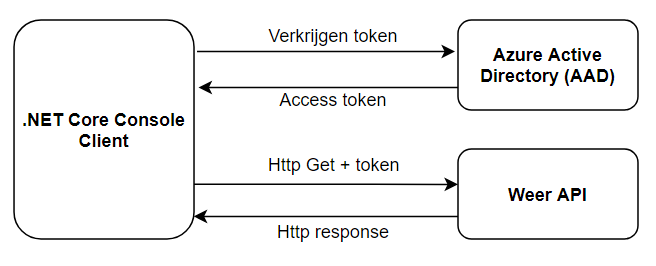
\includegraphics{POC_Final} 
	\caption[Dit is het eindresultaat van dit hoofdstuk]{Dit is het eindresultaat van dit hoofdstuk.}
	\label{fig:pocfinal}
\end{figure}
In deze proof of concept wordt gebruik gemaakt van:	
\begin{itemize}
	\item NET Core SDK 3.1
	\item Text Editor (recommended VS code)
	\item Azure Account (Free)
\end{itemize}
\subsection{\IfLanguageName{dutch}{Aanmaken API}{Making the API}}
Zoals eerder vermeld wordt er in deze proof of concept gebruik gemaakt van een weervoorspelling API. Om deze te gaan aanmaken kan er gebruik gemaakt worden van een NET Core SDK 3.1 template. Met VS code kan er in de terminal het volgende commando ingegeven worden: \emph{dotnet new webAPI -n weerAPI}.\newline
Na dit command ziet het schema er als volgt uit (figuur \ref{fig:poc1}). Deze template heeft een simpele controller met een GET methode die vijf willekeurige weersvoorspellingen zal teruggeven. Het aanmaken van de API houdt dan ook niet meer in dan deze simpele stap.
\begin{figure}[H]
	\centering
	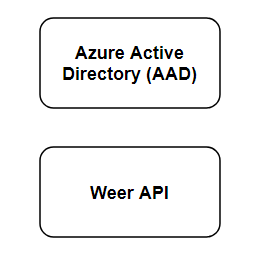
\includegraphics{POC1} 
	\caption[BeginPOC]{Begin vorm van de proof of concept.}
	\label{fig:poc1}
\end{figure}
\subsection{\IfLanguageName{dutch}{API registreren op Azure}{Registering the API on Azure}}
Nu de API aangemaakt is moet deze bekend gemaakt worden aan Azure active directory. Om dit te doen wordt gebruikt gemaakt van het Azure portal. In het overzicht gaat de gebruiker naar Azure active directory (figuur \ref{fig:azure1}).
\begin{figure}[H]
	\centering
	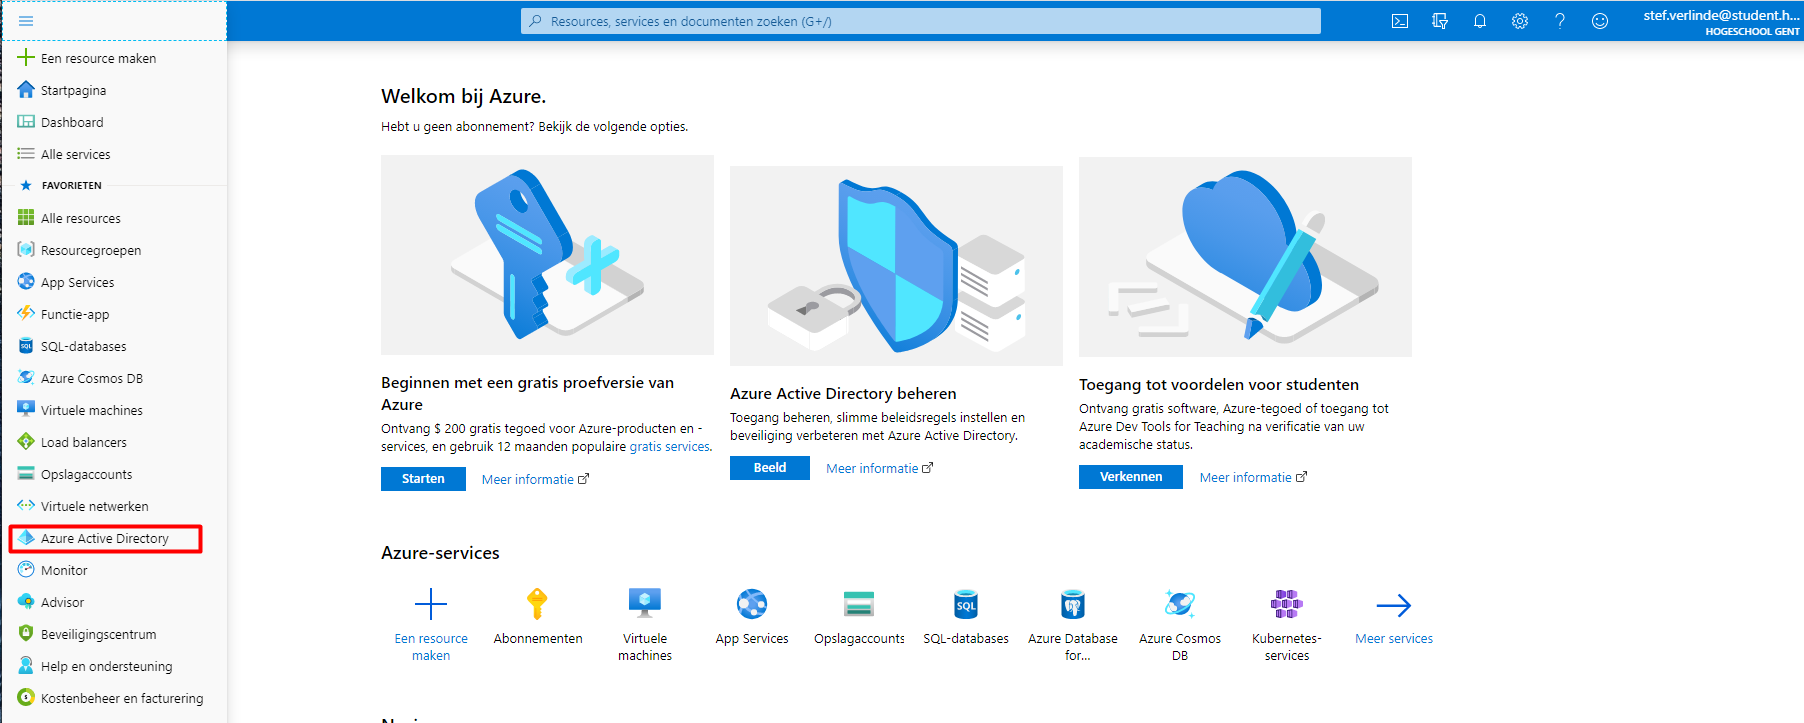
\includegraphics[scale=0.40]{Azure1} 
	\caption[BeginAzure]{Stap 1 in het toevoegen van de API.}
	\label{fig:azure1}
\end{figure}
Om de weervoorspelling API te registreren bij de active directory wordt in het overzicht genavigeerd naar “App-registraties” (figuur \ref{fig:azure2}).
\begin{figure}[H]
	\centering
	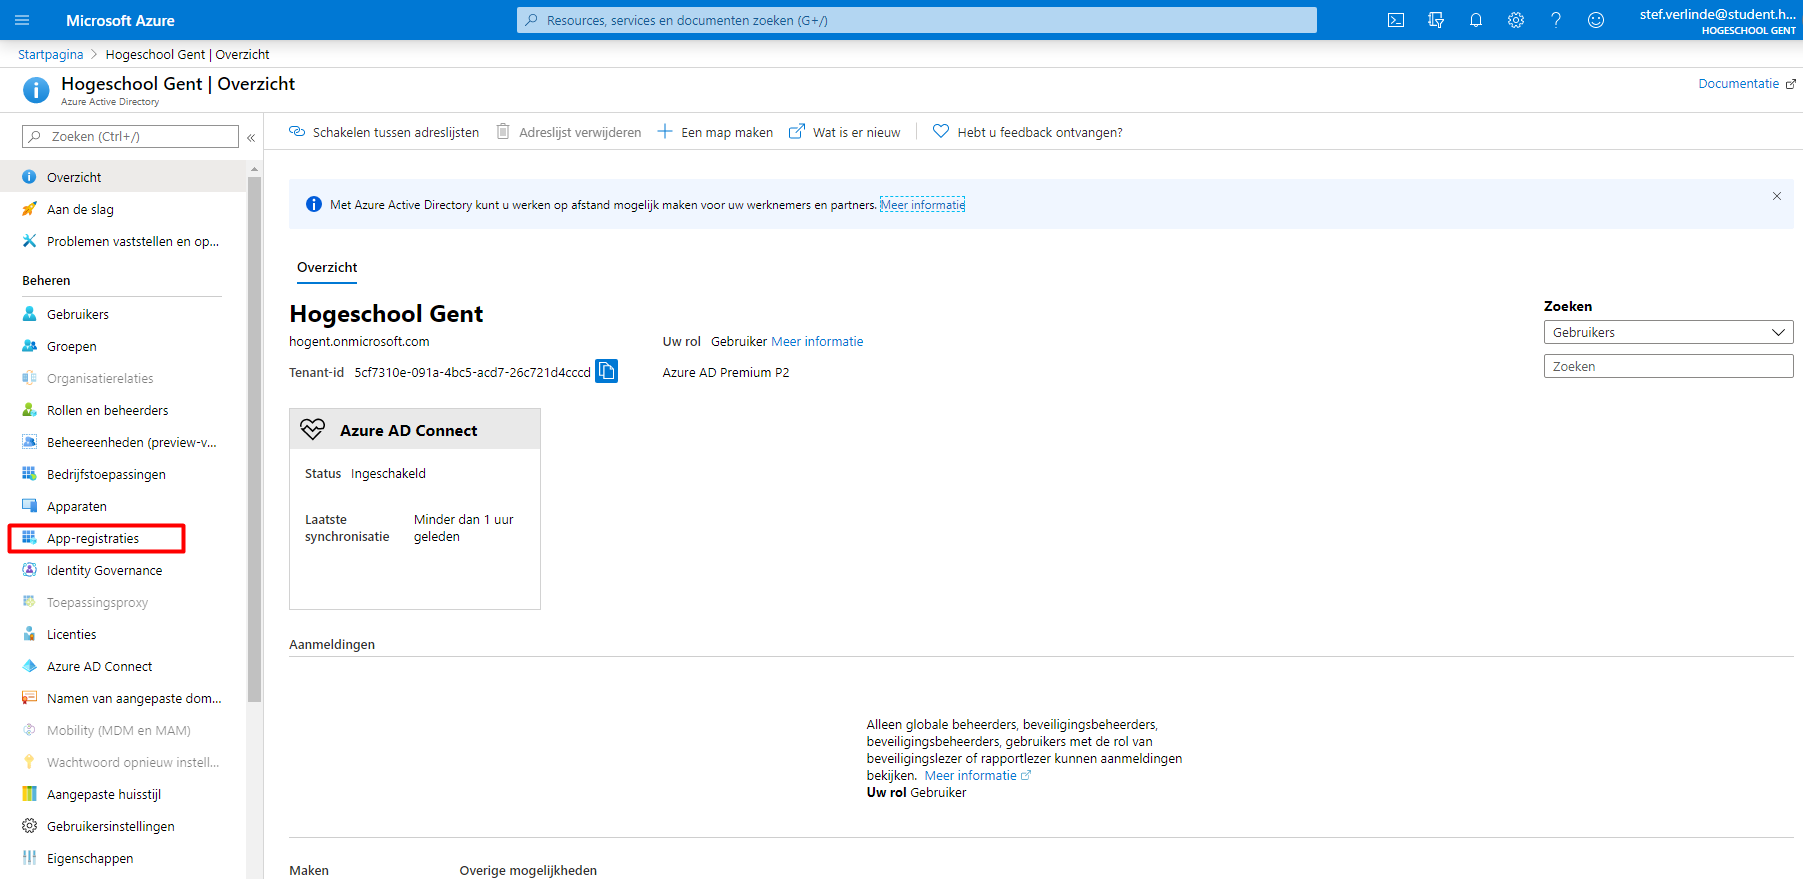
\includegraphics[scale=0.40]{Azure2} 
	\caption[Azure2]{Stap 2 in het toevoegen van de API.}
	\label{fig:azure2}
\end{figure}
In dit overzicht hebben gebruikers de mogelijkheid nieuwe apps te gaan registeren. Hier wordt dus via de knop “Nieuwe registratie” de weervoorspelling API toegevoegd (figuur \ref{fig:azure3}).
\begin{figure}[H]
	\centering
	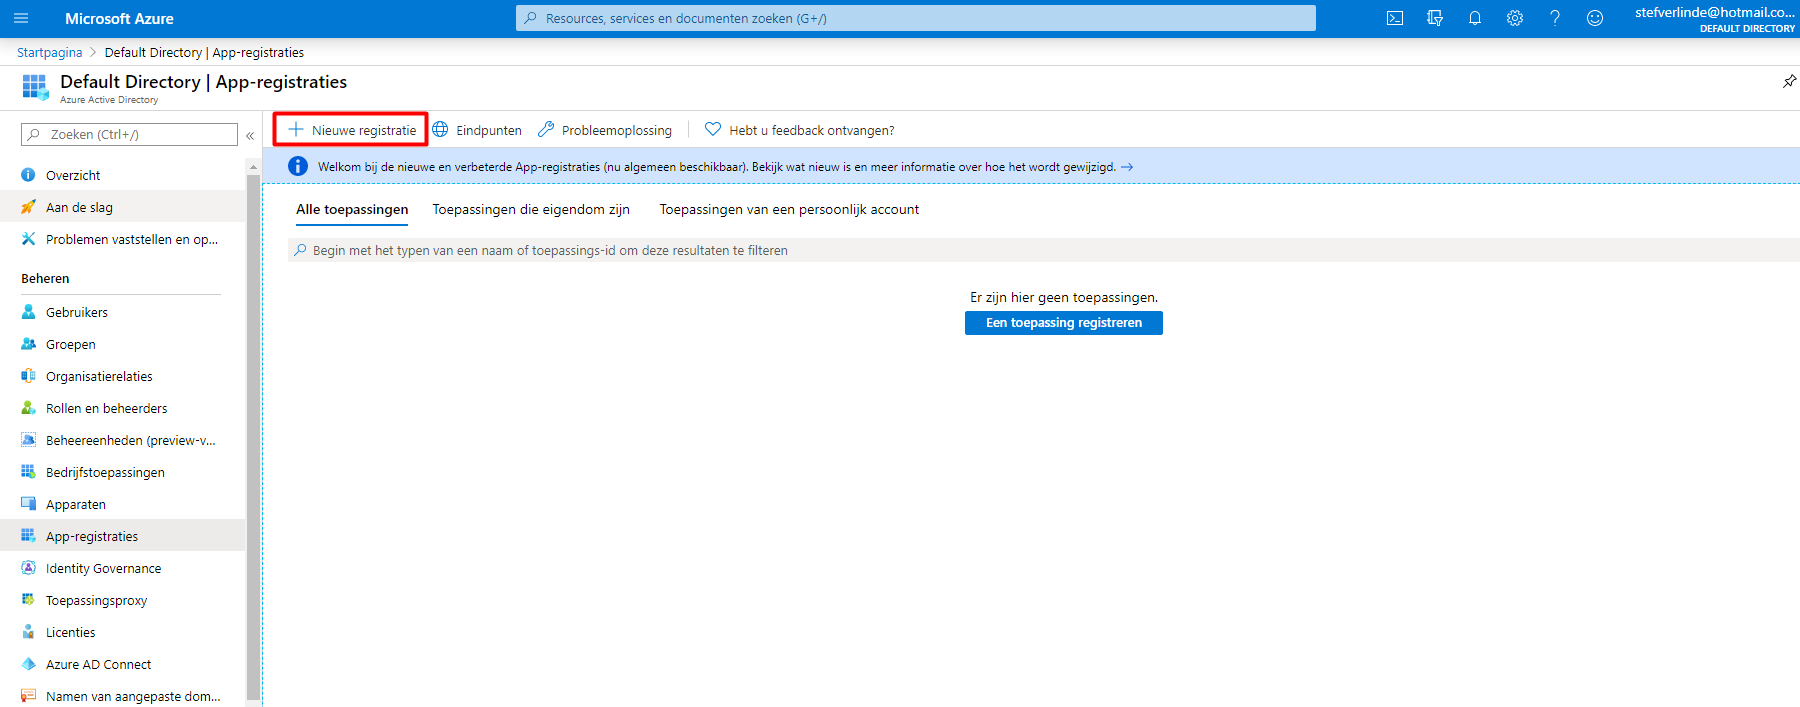
\includegraphics[scale=0.40]{Azure3} 
	\caption[Azure3]{Stap 3 in het toevoegen van de API.}
	\label{fig:azure3}
\end{figure}
In het volgende scherm krijgt de gebruiker de mogelijkheid om een naam in te geven voor de applicatie. In dit geval vult de gebruiker hier in “weerAPI”. De overige instellingen kunnen eventueel aangepast worden als de gebruiker wenst dat de API ook toegankelijk is voor accounts buiten de directory, bijvoorbeeld bij een business-to-businesssituatie. Hier kan ook een redirect-uri of omleidings-uri opgegeven worden. Als hier een uri wordt opgegeven dan wordt nadat een user geverifieerd is het verificatieantwoord naar deze uri gestuurd. Dit wordt bijvoorbeeld gebruikt in de tweede proof of concept met implicit grant. In de client credentials proof of concept kunnen alle extra instellingen op de standaard waarden gelaten worden. Dit is te zien in figuur \ref{fig:azure4}
\begin{figure}[H]
	\centering
	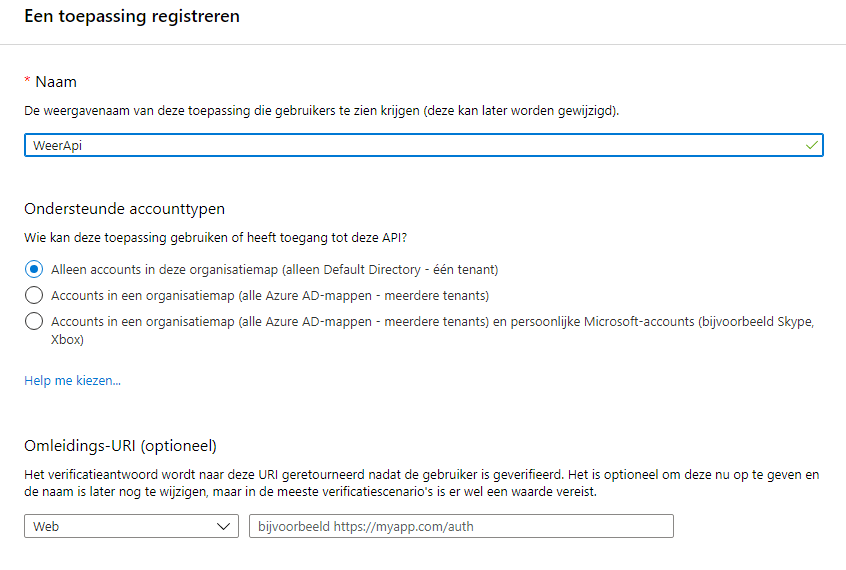
\includegraphics[scale=0.75]{Azure4} 
	\caption[Azure4]{Stap 4 in het toevoegen van de API.}
	\label{fig:azure4}
\end{figure}\newpage
Wanneer de API geregistreerd is binnen de active directory zijn er enkele belangrijke waarden die zichtbaar worden. Deze zijn de client ID en tenant ID. De client ID is een unieke GUID voor de API die net geregistreerd werd. De tenant ID is een unieke GUID voor onze active directory. Als een gebruiker binnen dezelfde active directory meerdere applicaties zou registreren dan zal deze tenant ID bij elke applicatie dezelfde zijn. Deze waarden zie je in figuur \ref{fig:azure5}.
\begin{figure}[H]
	\centering
	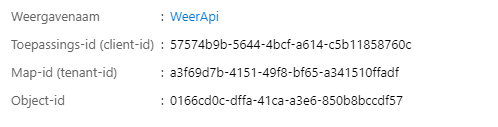
\includegraphics{Azure5} 
	\caption[Azure5]{Belangrijke waarden na het aanmaken van de API.}
	\label{fig:azure5}
\end{figure} 
De volgende stap is het aanmaken van een applicatie ID of resource ID. Dit wordt gedaan om aan Azure duidelijk te maken dat deze API gebruikt zal worden. De API wordt geëxposeerd of beschikbaar gemaakt aan Azure (figuur \ref{fig:azure6}).
\begin{figure}[H]
	\centering
	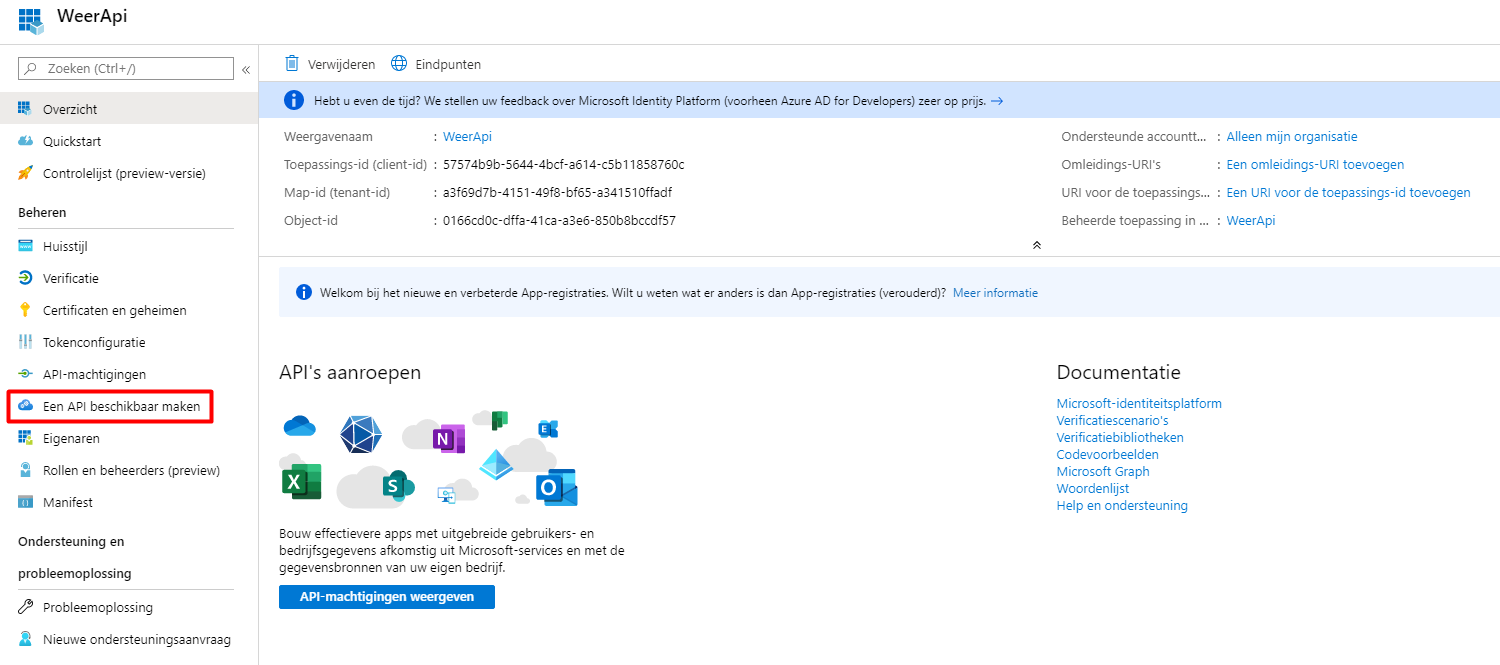
\includegraphics[scale=0.50]{Azure6} 
	\caption[Azure6]{Stap 5 in het toevoegen van de API.}
	\label{fig:azure6}
\end{figure}
Bij “Een API beschikbaar stellen” wordt op de knop “instellen” geklikt en daarna op “opslaan”. Deze stappen worden afgebeeld in figuur \ref{fig:azure7} en \ref{fig:azure8}. Hierdoor wordt er een resource ID aangemaakt. Dit resource ID is nu ook zichtbaar in het overzicht van de API-applicatie (figuur \ref{fig:azure9}).
\begin{figure}[H]
	\centering
	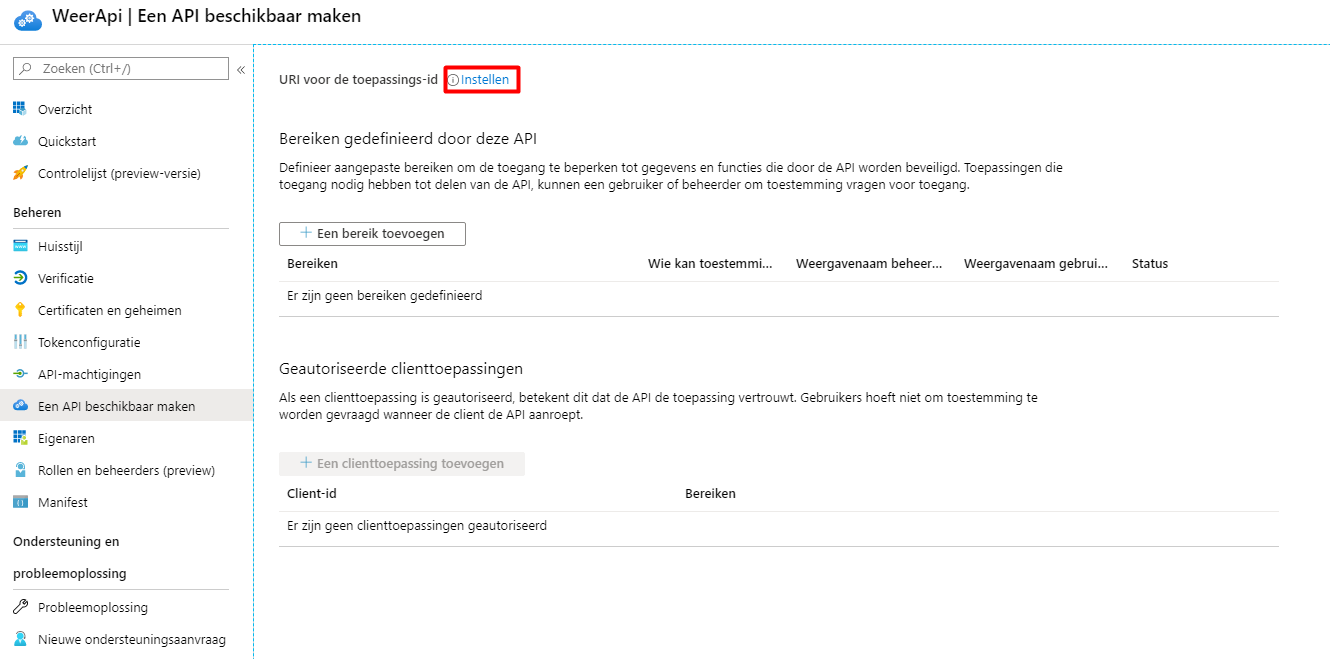
\includegraphics[scale=0.50]{Azure7} 
	\caption[Azure7]{Stap 6 in het toevoegen van de API.}
	\label{fig:azure7}
\end{figure}
\begin{figure}[H]
	\centering
	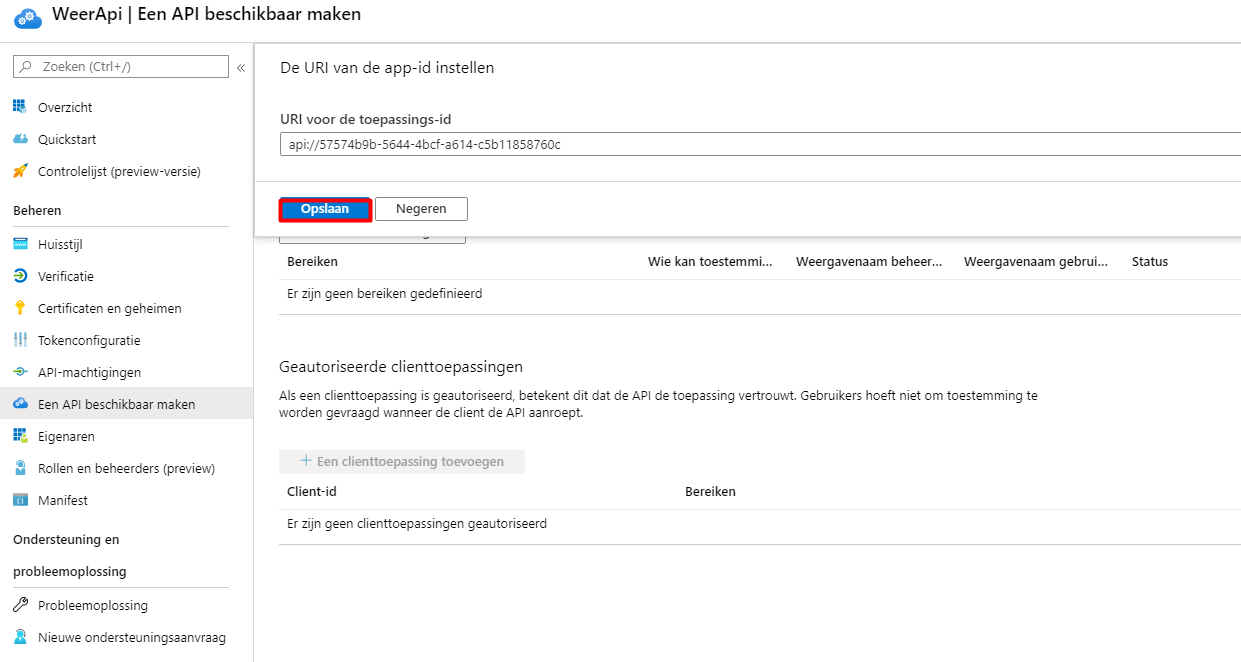
\includegraphics[scale=0.50]{Azure8} 
	\caption[Azure8]{Stap 7 in het toevoegen van de API.}
	\label{fig:azure8}
\end{figure}
\begin{figure}[H]
	\centering
	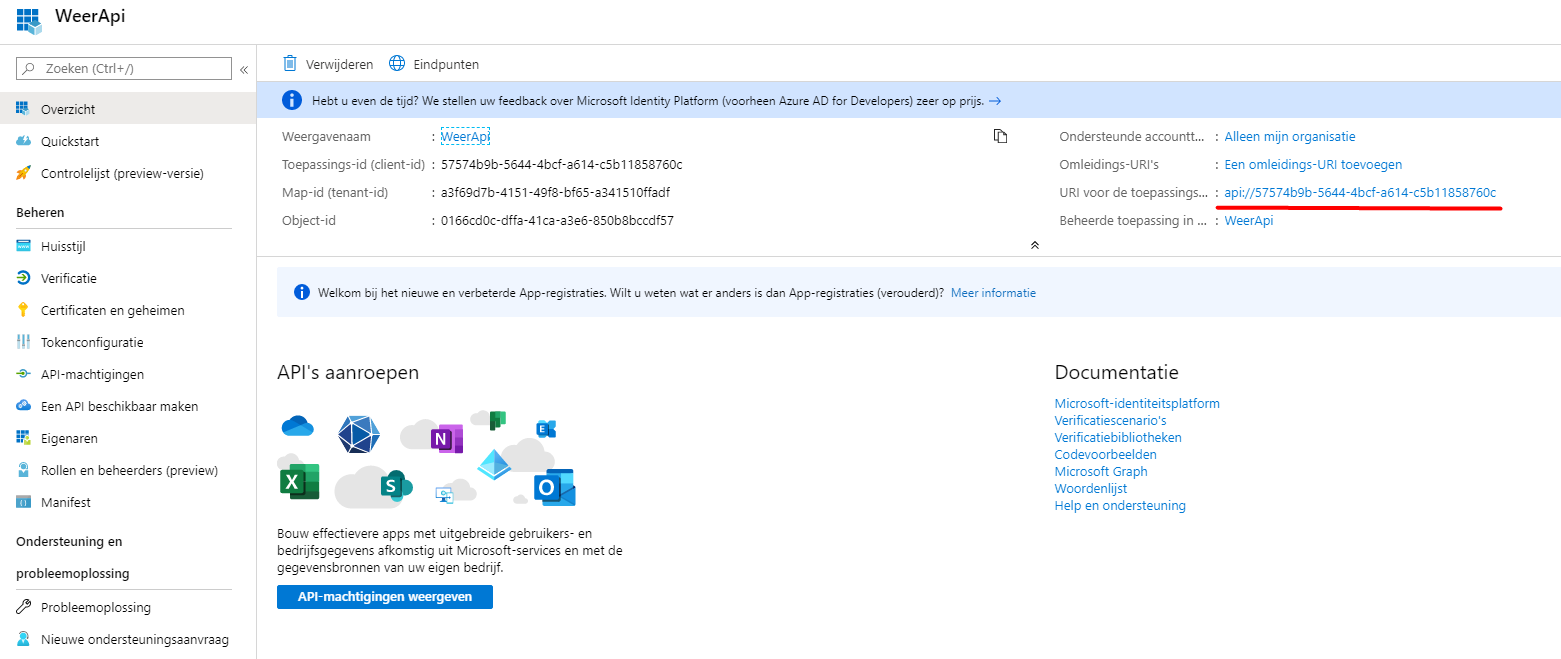
\includegraphics[scale=0.40]{Azure9} 
	\caption[Azure9]{Hier wordt nu het resource ID getoond.}
	\label{fig:azure9}
\end{figure}\newpage
De laatste stap in het registreren van de API-applicatie is het wijzigen van het manifest. Een manifest is niks meer dan een json-file. In deze json-file kan een gebruiker aan Azure vertellen wat voor type applicatie toegang heeft tot de API. \newline
In deze json-file zal de gebruiker de “appRoles” array moeten aanpassen zoals in figuur \ref{fig:azure10}. Hier kan een gebruiker verschillende configuraties ingeven. Belangrijk hier is dat ID een geldige GUID moet zijn. De waarde voor value is welke applicatie role toegang krijgt tot de API.
\begin{figure}[H]
	\centering
	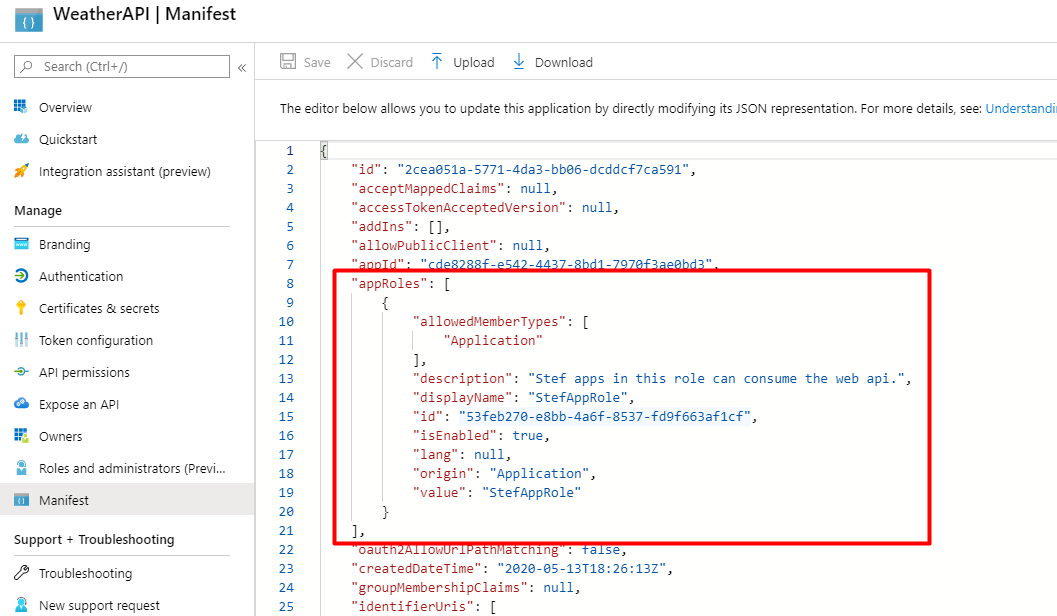
\includegraphics[scale=0.60]{Azure10} 
	\caption[Azure10]{Stap 8 in het toevoegen van de API.}
	\label{fig:azure10}
\end{figure}
\subsection{\IfLanguageName{dutch}{Connectie API en AAD}{Connection API and AAD}}
Nu de API geregistreerd is in Azure active directory kan de gebruiker de momenteel nog aparte API implementatie en registratie op Azure verbinden. Dit gebeurt door het resource ID, tenant ID en instance ID van de Azure API op te slaan in de API implementatie. Voor demonstratiedoeleinden worden deze hier opgeslagen in de appsettings.json file van het API project (figuur \ref{fig:appsetAPI}). Als de gebruiker wenst deze proof of concept in development te gaan gebruiken wordt aangeraden deze gevoelige informatie in een user secret of key vault te plaatsen.
\begin{figure}[H]
	\centering
	\includegraphics{appsettingsAPI} 
	\caption[Appsetingsjosn]{Appsettings.json-file van de API.}
	\label{fig:appsetAPI}
\end{figure}
Deze waarden kunnen nu gebruikt worden om de connectie tussen de implementatie en Azure-registratie te voltooien. Aangezien de beveiliging van de API aan de hand van jwt bearer tokens gebeurt gebruikt men het resource ID als audience en de instance en tenant ID’s als authority. De code voor in de startup classe zie je in figuur \ref{fig:configureServices} en \ref{fig:configure}. 
\begin{figure}[H]
	\centering
	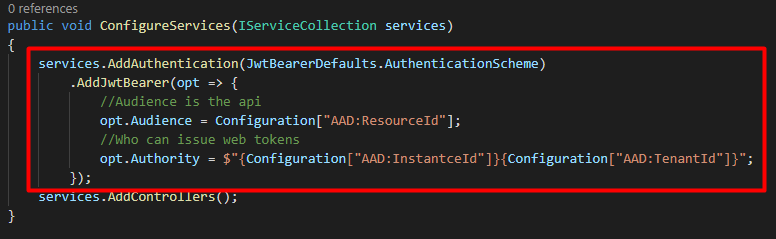
\includegraphics{ConfigureServices} 
	\caption[ConfigureServices]{ConfigureServices methode van de API.}
	\label{fig:configureServices}
\end{figure}\newpage
\begin{figure}[H]
	\centering
	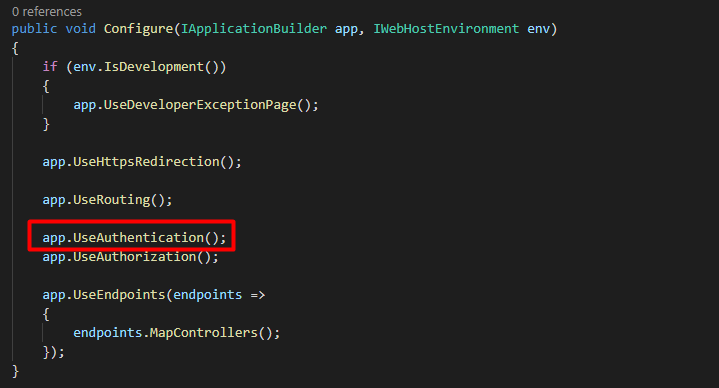
\includegraphics{Configure} 
	\caption[Configure]{Configure methode van de API.}
	\label{fig:configure}
\end{figure}
Laatste stap is het toevoegen van een Authorize attribute aan de endpointmethode. Zo kan deze methode enkel aangeroepen worden door een geverifieerde client. Een niet geverifieerde client krijgt dan een 401 unauthorized error.
\subsection{\IfLanguageName{dutch}{Client registreren op azure}{Registering client on Azure}}
Op een gelijkaardige manier kan ook een client geregistreerd worden bij Azure. In het overzicht “App-registraties” van Azure active directory kan men nu een nieuwe client toevoegen (figuur \ref{fig:azure11}).
\begin{figure}[H]
	\centering
	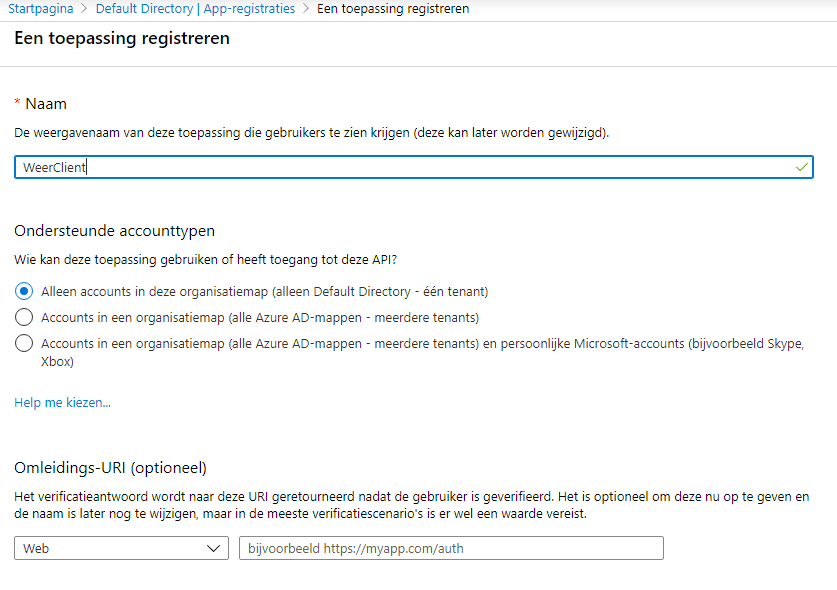
\includegraphics[scale=0.60]{Azure11} 
	\caption[Azure11]{Stap 1 in het registreren van de client.}
	\label{fig:azure11}
\end{figure}
Na het aanmaken van deze client worden de client- en tenant-ID’s opnieuw zichtbaar. Hier valt op dat zoals eerder vermeld het tenant-ID hetzelfde is als bij de weerAPI. De volgende stap is het opzetten van een client secret. Een client secret wordt door de client naar Azure gestuurd om te bewijzen dat de client is wie hij zegt dat hij is. Een client secret is discrete informatie en daar moet voorzichtig mee omgegaan worden. In het active directory overzicht bij “Certificaten en geheimen” kan een secret worden toegevoegd (figuur \ref{fig:azure12} en \ref{fig:azure13}). 
\begin{figure}[H]
	\centering
	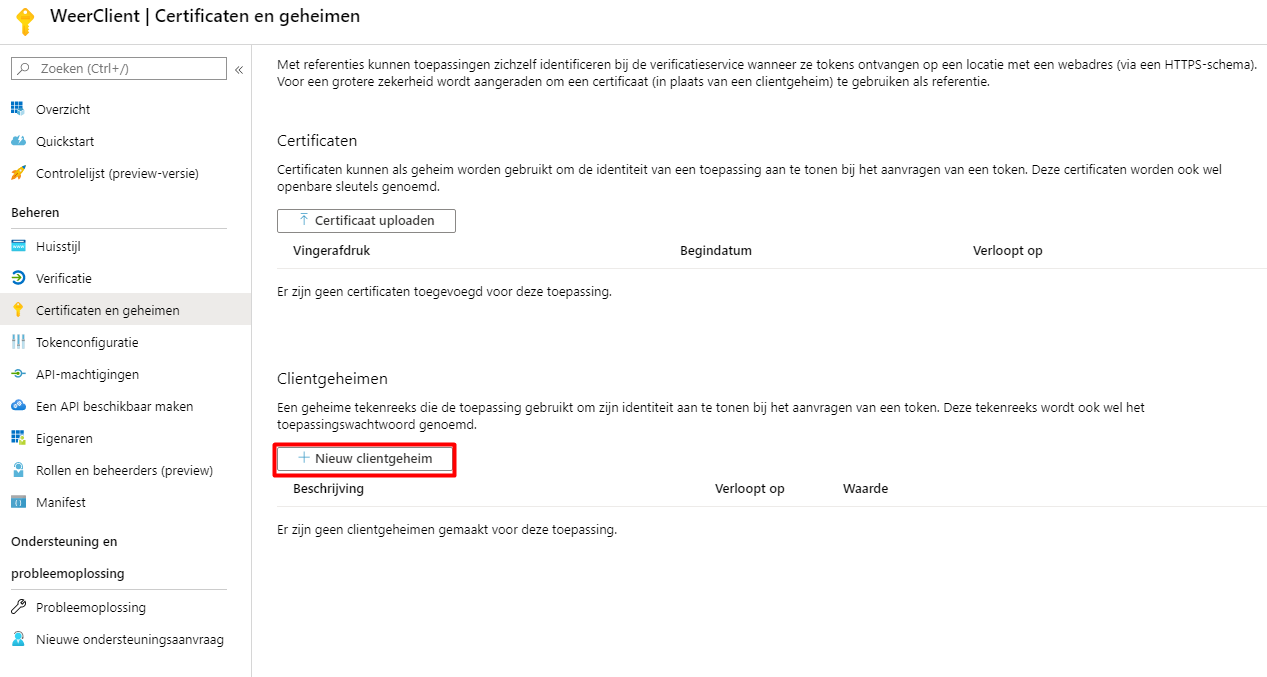
\includegraphics[scale=0.60]{Azure12} 
	\caption[Azure12]{Stap 2 in het registreren van de client.}
	\label{fig:azure12}
\end{figure}
\begin{figure}[H]
	\centering
	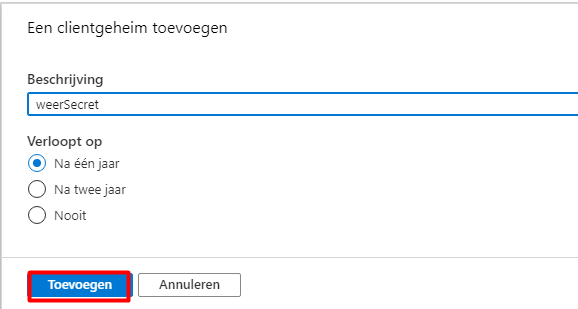
\includegraphics{Azure13} 
	\caption[Azure13]{Stap 3 in het registreren van de client.}
	\label{fig:azure13}
\end{figure}
De laatste stap voor de client is duidelijk maken welke permissions de client heeft tegenover de API. Dit kan ingesteld worden via het overzicht “API-permissions”. Bij het klikken op machtiging toevoegen valt op dat onder “mijn API’s” de zelf aangemaakte API van de gebruiker terug te vinden is. Na het klikken op de API valt op dat er een keuze is tussen twee machtigingen of permissions: gedelegeerde machtigingen en toepassingsmachtigingen. Aangezien er in deze proof of concept een daemon client gebruikt wordt, ofwel een client zonder input van een gebruiker, kiezen we voor toepassingsmachtigingen. Hierna wordt op de role geklikt die in de manifest json-file van de API geconfigureerd is (figuur \ref{fig:azure14}). 
\begin{figure}[H]
	\centering
	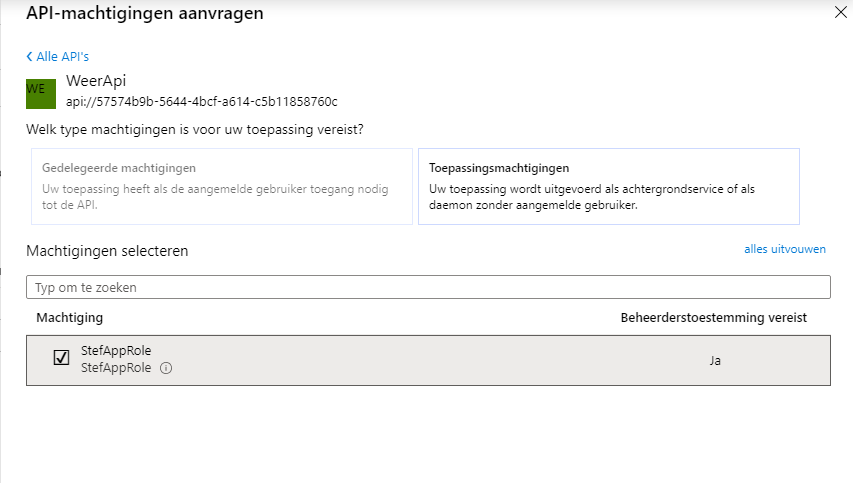
\includegraphics[scale=0.85]{Azure14} 
	\caption[Azure14]{Stap 4 in het registreren van de client.}
	\label{fig:azure14}
\end{figure}
Na het toevoegen van de permission is er nog toestemming van de beheerder nodig om deze permission te activeren. Dit wordt gedaan door op “Beheerderstoestemming verlenen voor Default Directory” te klikken (figuur \ref{fig:azure15}).
\begin{figure}[H]
	\centering
	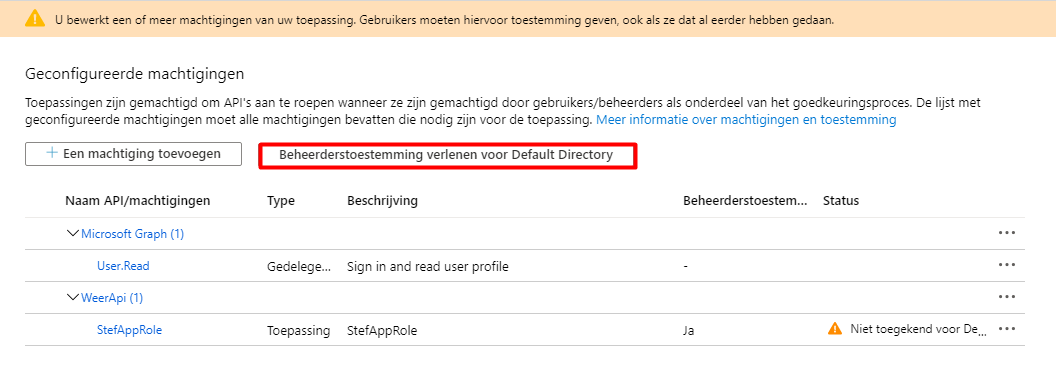
\includegraphics[scale=0.75]{Azure15} 
	\caption[Azure15]{Stap 5 in het registreren van de client.}
	\label{fig:azure15}
\end{figure}
\subsection{\IfLanguageName{dutch}{Aanmaken client applicatie}{Making the client applicatie}}
Gelijkaardig aan de API is het mogelijk met het volgende dotnet commando een console applicatie template genereren: \emph{dotnet new console -n weerClient}\newline
Schematisch wordt de flow na het aanmaken van de client als volgt afgebeeld (figuur \ref{fig:poc2}). Alles in Azure active directory staat al klaar voor de communicatie maar hiervoor moet de configuratie in de client in orde gebracht worden.
\begin{figure}[H]
	\centering
	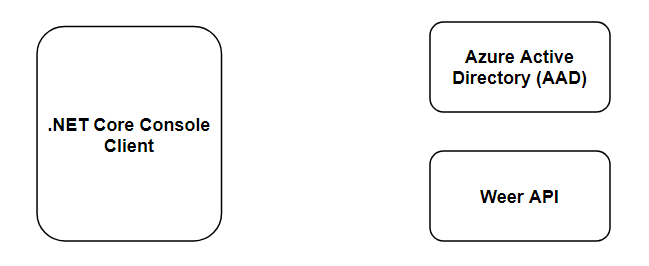
\includegraphics{POC2} 
	\caption[POC2]{Na het maken van de client kan het schema als volgt worden aangevuld.}
	\label{fig:poc2}
\end{figure}
Net zoals in de API-applicatie is het belangrijk dat de client op de hoogte is van enkele waarden uit Azure active directory. Deze zijn de instance, tenant ID, client ID, de gemaakte client secret en het basisadres van de API (figuur \ref{fig:appsettingsClient}). In dit voorbeeld ziet dit er als volg uit. Ook hier is het belangrijk om te begrijpen dat dit enkel in appsettings wordt opgeslagen voor demonstratiedoeleinden. In een development omgeving zouden client secrets in een key vault opgeslagen worden.
\begin{figure}[H]
	\centering
	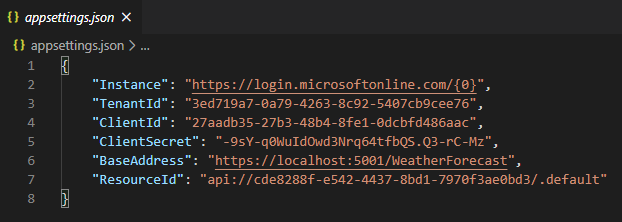
\includegraphics{appsettingsClient} 
	\caption[POC2]{appsettings.json-file in de client applicatie.}
	\label{fig:appsettingsClient}
\end{figure}
Omdat appsettings een json-file is, heeft de consoleapplicatie een manier nodig om deze te kunnen inlezen. Om dit te vergemakkelijken wordt er een AuthConfig klasse aan gemaakt met alle attributen die nodig zijn om de Azure connectie te maken (figuur \ref{fig:authConfig}).
\begin{figure}[H]
	\centering
	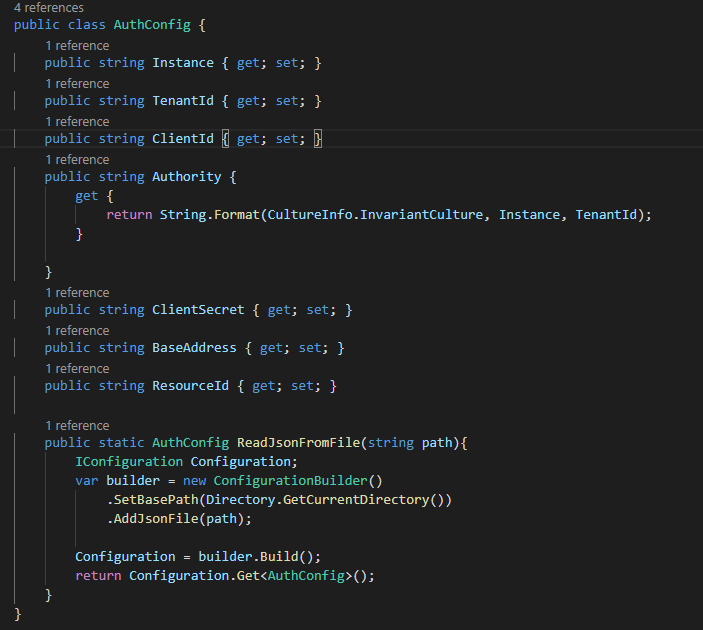
\includegraphics{AuthConfig} 
	\caption[AuthConfig]{AuthConfig klasse in de client.}
	\label{fig:authConfig}
\end{figure}\newpage
Vanaf nu is alles aanwezig om een connectie met Azure te maken. In dit voorbeeld doen we dit als volgt. De eerste connectie die de client moet maken is een geldige token vragen aan Azure active directory. In figuur \ref{fig:aquireToken} zien we dat eerst de waarden uit het appsetingsbestand gelezen worden. Daarna wordt een ConfidentialClient aangemaakt met het voorziene client ID, client secret en de authority. Er is ook een array van resource ID’s. Deze heeft in dit voorbeeld enkel de weervoorspelling API als resource vandaar dat hier het resource ID van deze API inkomt. De volgende try block haalt de token op voor de client van de resource en print deze uit.
\begin{figure}[H]
	\centering
	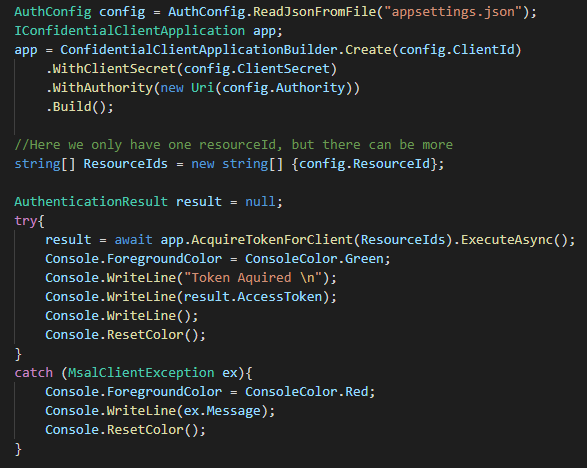
\includegraphics{AquireToken} 
	\caption[AuthConfig]{Deze code toont het ophalen van de access token door de client.}
	\label{fig:aquireToken}
\end{figure}\newpage
Na het uitvoeren van deze code is volgende connectie succesvol gelegd. Een client, in dit geval de weervoorspelling client, kan nu een access token ophalen van de Azure active directory.
\begin{figure}[H]
	\centering
	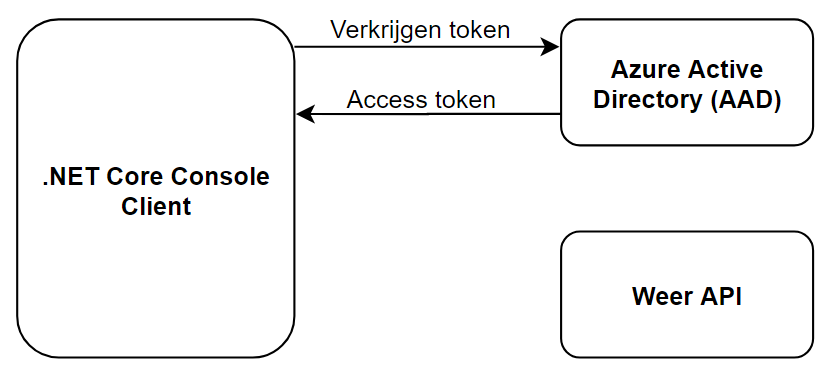
\includegraphics[scale=0.55]{POC3} 
	\caption[POC3]{Hier wordt schematisch afgebeeld dat de client nu een access token van AAD kan ophalen.}
	\label{fig:poc3}
\end{figure}
Om het schema compleet te maken moet de client met deze access token om de API data vragen. Als deze access token correct is zal de client de weervoorspellinggegevens krijgen. In deze proof of concept gebeurt dit als volgt.\newline
Ten eerste wordt gecheckt of er een access token van Azure active directory aanwezig is. Daarna wordt er een httpClient aangemaakt en wordt er gecheckt of de defaultRequestHeaders het media type json accepteren. Daarna wordt het  type op bearer gezet en wordt er een GET methode naar de API gestuurd. Als de response succesvol is wordt deze uitgeprint, zo niet wordt de errorboodschap getoond (figuur \ref{fig:aquireData}).
\begin{figure}[H]
	\centering
	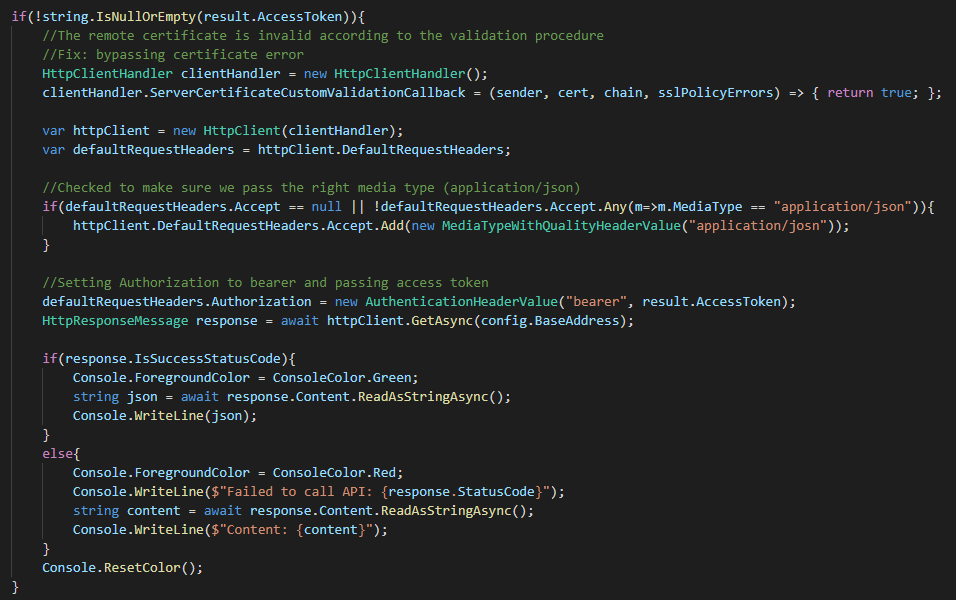
\includegraphics[scale=0.70]{AquireData} 
	\caption[AquireData]{Deze code toont het ophalen van data aan de hand van een access token op de API.}
	\label{fig:aquireData}
\end{figure}\newpage
Door deze code is het schema compleet en kan de client met een access token van Azure active directory aan de data van de API.
\begin{figure}[H]
	\centering
	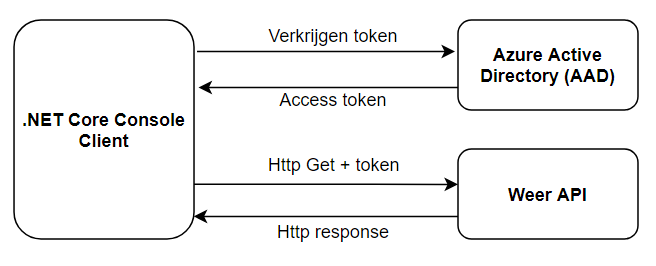
\includegraphics{POC_Final} 
	\caption[POCFinal2]{Op dit schema is het eindresultaat te zien.}
	\label{fig:pocfinal2}
\end{figure}
\section{\IfLanguageName{dutch}{Proof of concept met implicit grant type}{Proof of concept with implicit grant type}}
\label{sec:Microsift_signon}
Het verschil met client credential grant authentication en implicit grant authentication is dat er bij implicit grant input van de gebruiker verwacht wordt. Namelijk een gebruikersnaam en wachtwoord, hierdoor zijn er enkele extra stappen in de flow voor de authentication. Bij client credential grant is er geen input van de gebruiker, zoals gezien in de eerste proof of concept (POC \cite{Verlinde2020}).
\subsection{\IfLanguageName{dutch}{Registratie in azure}{Registration in Azure}}
Om een client met implicit grant authentication toe te voegen aan de Azure active directory gaat de gebruiker naar “App-registraties” in de Azure portal bij active directory. Hier wordt opnieuw een nieuwe client toegevoegd met de knop “Nieuwe registratie”. Als naam wordt hier “SignOnClient” genomen, de andere instellingen houden we op de default instellingen (figuur \ref{fig:azure16}). 
\begin{figure}[H]
	\centering
	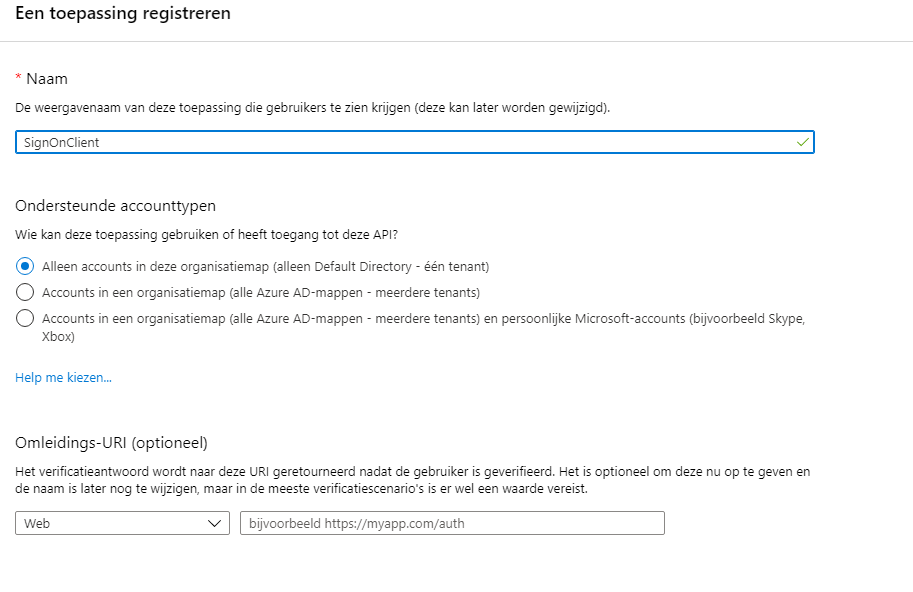
\includegraphics[scale=0.75]{Azure16} 
	\caption[Azure16]{Stap 1 in het registreren van de client met implicit grant.}
	\label{fig:azure16}
\end{figure}
Na het aanmaken van de client is het mogelijk om bij ”Quickstart” makkelijk de client te configureren. Hier worden er enkele mogelijkheden voorgesteld door Azure voor het opstarten van de client. In deze proof of concept werd er gekozen voor een .NET Core webtoepassing (figuur \ref{fig:azure17} en \ref{fig:azure18}).
\begin{figure}[H]
	\centering
	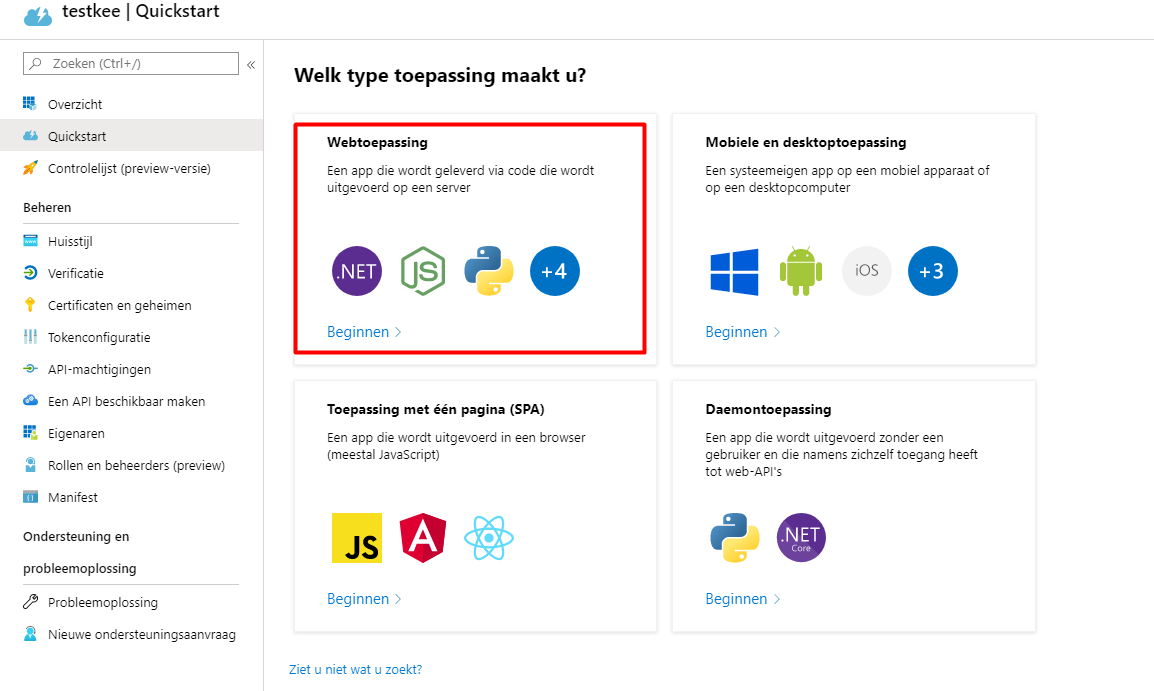
\includegraphics[scale=0.60]{Azure17} 
	\caption[Azure17]{Stap 2 in het registreren van de client met implicit grant.}
	\label{fig:azure17}
\end{figure}\newpage
\begin{figure}[H]
	\centering
	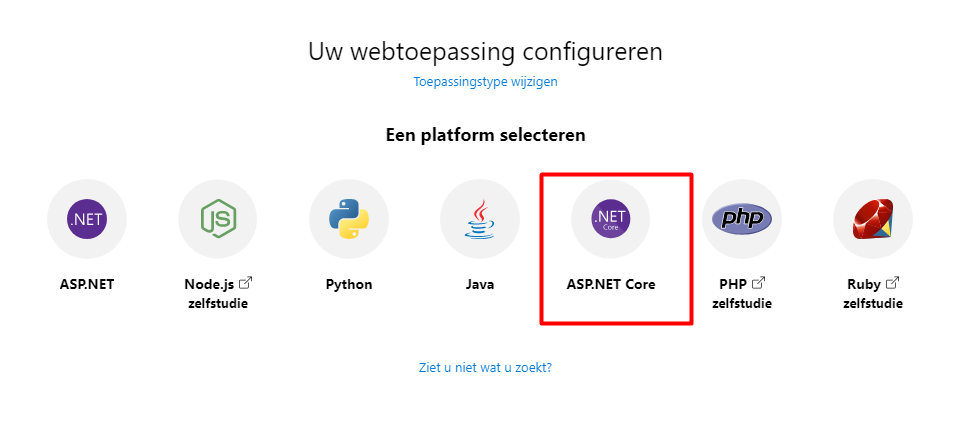
\includegraphics[scale=0.60]{Azure18} 
	\caption[Azure18]{Stap 3 in het registreren van de client met implicit grant.}
	\label{fig:azure18}
\end{figure}
In het laatste scherm van de quickstart worden er door Azure enkele stappen voorgelegd. Bij stap 1 moeten er enkele URLs opgegeven worden, dit zijn de redirect URLs en postLogout URLs. Onder deze stap is er ook een knop om dit Azure automatisch te laten doen zodat de gebruiker dit zelf niet moet invullen. Deze automatische invulling is ook wat in deze proof of concept gebruikt is. Stap 2 is om de quickstart te downloaden. Na het downloaden en starten van de client zou het inloggen met een Microsoft-account al moeten werken.\newline\newline
Het verschil tussen een implicit grant authentication en client credential grant authentication bevindt zich dus in de flow van de tokens. Zoals in het schema van de flow gezien wordt zijn er bij implicit grant enkele extra stappen vereist. In deze proof of concept wordt er eerst naar de .NET Core applicatie gegaan, maar het request zal meteen doorgestuurd worden naar de Microsoft identity server. Hier zal de gebruiker zijn gegevens moeten ingeven om zo aan een geldige access token te komen. Na deze stap wordt met de redirectURL teruggegaan naar de .NET Core applicatie en kan de pagina geladen worden. Omdat we bij het aanmaken van de client in Azure ervoor gekozen hebben dat deze client enkel toegankelijk mocht zijn voor users binnen de organisatiemap zullen enkel Microsoft accounts binnen de Azure active directory toegang hebben na het inloggen. Een schematische voorstelling van de token flow kan gezien worden in figuur \ref{fig:signOn}. 
\begin{figure}[H]
	\centering
	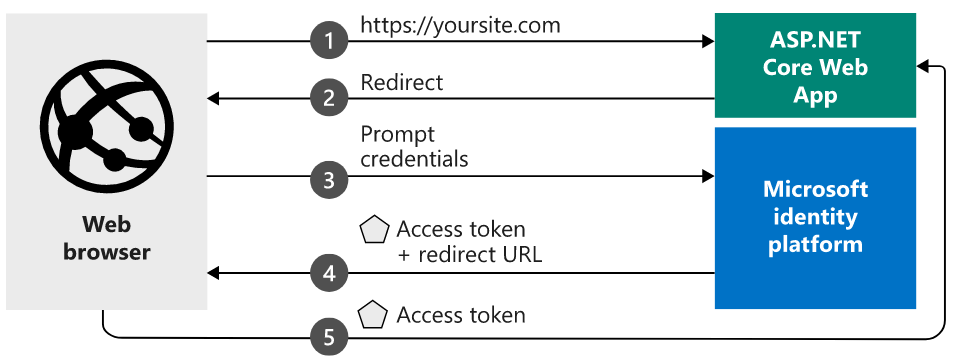
\includegraphics[scale=0.65]{SignOn} 
	\caption[SignOn]{Schematische voorstelling van de implicit grant flow.}
	\label{fig:signOn}
	\scriptsize
	\cite{jmprieur2019}
\end{figure}
\section{\IfLanguageName{dutch}{Authorization Code grant}{Authorization Code grant}}
\label{sec:authorizationCode}
Na de proof of concepts van client credential grant en implicit grant uit te klaren is het zeker ook belangrijk om naar de authorization code grant te kijken. Een schematische voorstelling van de authorzation code grant ziet er als volgt uit (figuur \ref{fig:authGrant1}).
\begin{figure}[H]
	\centering
	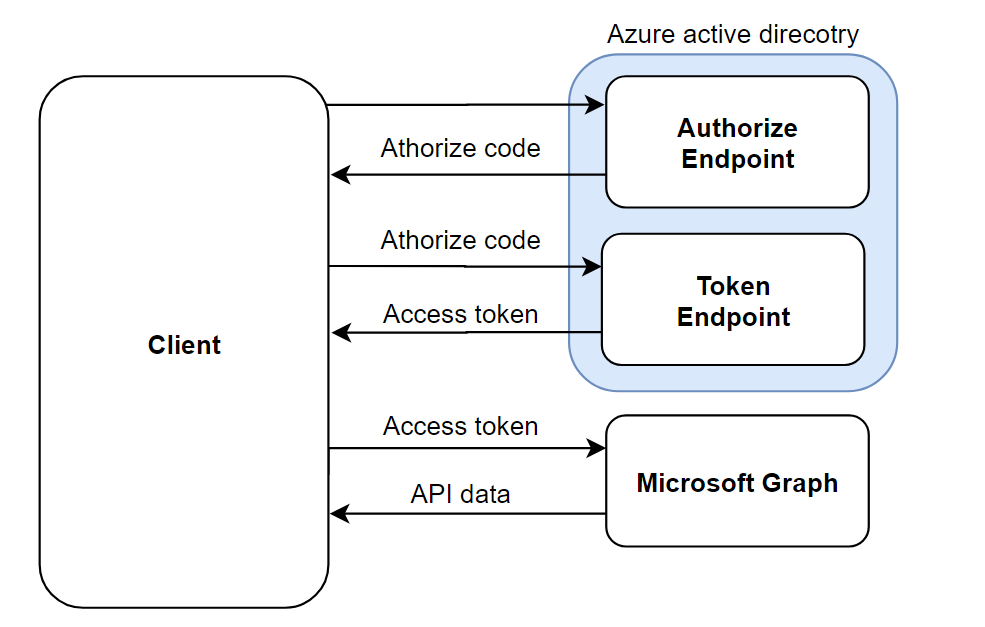
\includegraphics[scale=0.80]{AuthorizationGrant1} 
	\caption[AthorizationGrant1]{Schematische voorstelling van de authorization code grant flow.}
	\label{fig:authGrant1}
	\scriptsize
\end{figure}
\subsection{\IfLanguageName{dutch}{Code grant flow}{Code grant flow}}
Om deze flow uit te testen wordt gebruik gemaakt van het programma Postman om een request te sturen naar de Azure active direcotry beschermde API Microsoft graph. Deze connectie zal in dit voorbeeld handmatig ingegeven worden om de flow op een dieper level te bekijken. Om te beginnen wordt een nieuwe applicatie geregistreerd in Azure active direcotry. Opnieuw wordt gekozen voor single tenant account types en bij redirect URI wordt voor "web" gekozen met de URL "https://localhost" (figuur \ref{fig:authGrant2}).\newpage
\begin{figure}[H]
	\centering
	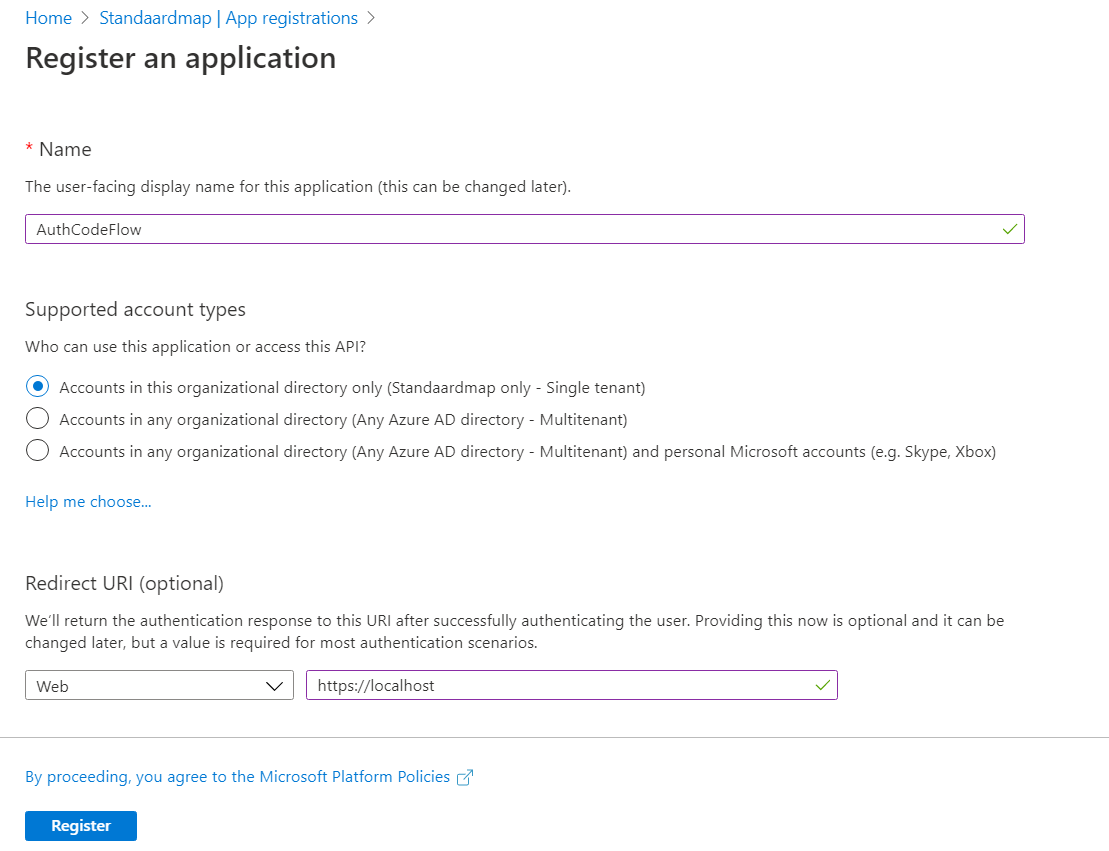
\includegraphics[scale=0.75]{AuthorizationGrant2} 
	\caption[AthorizationGrant2]{Registratie van een client voor authorization code grant.}
	\label{fig:authGrant2}
	\scriptsize
\end{figure}
Enige en laatste stap om de client te configureren is het aanmaken van een client secret. Dit gebeurt op gelijkaardige manier als in hoofdstuk \ref{sec:Client_Credentials_Grant}. Om aan een geldige access token te komen via deze client moeten er geen extra instellingen gewijzigd worden. Enkel de read permission zal nodig zijn om de flow te testen en deze wordt standaard aan een client gegeven door Azure active directory.\newline
De huidige situatie van de flow is de volgende. Als in Postman een request gestuurd wordt naar de API (Microsoft graph) dan wordt een body terug gestuurd met een boodschap "Access token is empty." en een status "401 Unauthorized". Dit komt omdat er momenteel nog geen acces token met het request wordt meegestuurd. Een voorbeeld hiervan zie je in figuur \ref{fig:authGrant3}.
\begin{figure}[H]
	\centering
	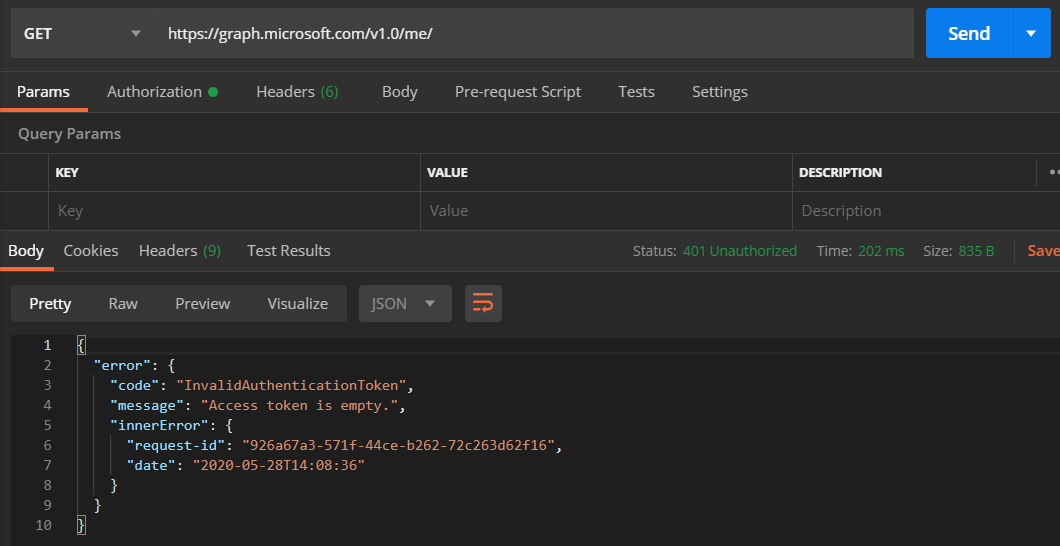
\includegraphics[scale=0.75]{AuthorizationGrant3} 
	\caption[AthorizationGrant3]{Voorbeeld van eerste request naar de API.}
	\label{fig:authGrant3}
	\scriptsize
\end{figure}
Om aan de data op de API te kunnen is er dus een geldige access token nodig. Deze connectie wordt met behulp van Postman handmatig ingegeven. Onder de tab Authorization bij \emph{Get new access} token worden al de nodige parameters getoond. Hier wordt als callback URL dezelfde URL als de redirect URL van de Azure client ingegeven. Bij Auth URL en Access token URL worden de URLs van Azure endpoints ingegeven. Client ID stelt het ID voor van de aangemaakt client in Azure. Als scope wordt de read scope gebruikt, dit kunnen ook andere scopes zijn. Een voorbeeld van de parameters zie je in figuur \ref{fig:authGrant4}.
\begin{figure}[H]
	\centering
	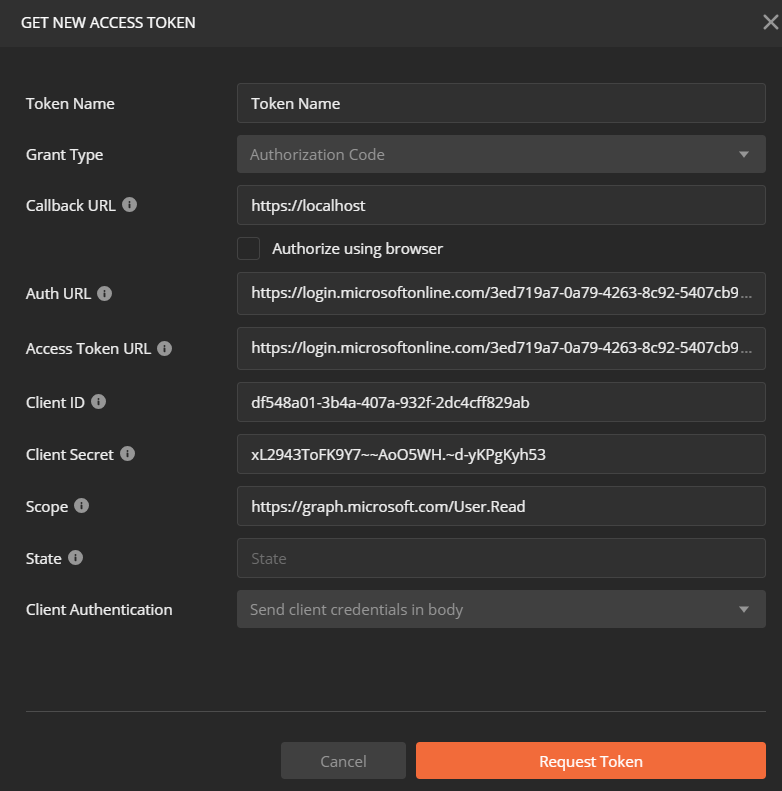
\includegraphics[scale=0.50]{AuthorizationGrant4} 
	\caption[AthorizationGrant4]{Parameters voor het aanvragen van een access token met authorization grant.}
	\label{fig:authGrant4}
	\scriptsize
\end{figure}
Wanneer met deze parameters een access token aangevraagd wordt moet worden ingelogd met een Microsoft account, daarna moeten de permissions geaccepteerd worden. Als dit goed gaat, wordt door Azure active directory een access token voorzien. Als de request opnieuw wordt uitgevoerd met deze token worden de data van de Microsoft graph API teruggestuurd (figuur \ref{fig:authGrant5}).
\begin{figure}[H]
	\centering
	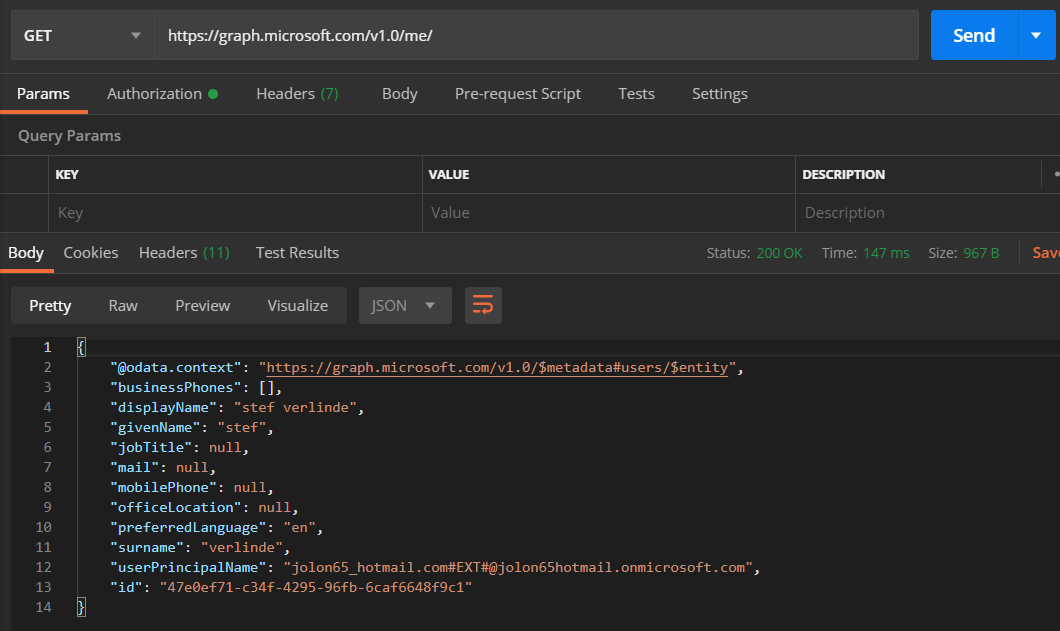
\includegraphics[scale=0.50]{AuthorizationGrant5} 
	\caption[AthorizationGrant5]{Resultaat van de call naar de API met access token.}
	\label{fig:authGrant5}
	\scriptsize
\end{figure}
\section{\IfLanguageName{dutch}{Vergelijking POC's}{Comparing POC's}}
\label{sec:comparePoc}
Na het bestuderen van zowel de client credential grant type die gebruikt maakt van applicatie access tokens, implicit grant type die gebruikt maakt van user access tokens en authorization grant type vallen enkele dingen op. Schematisch verschillen deze methoden niet erg veel. Wat welt opvalt is dat er bij auhorization code grant een extra call wordt gedaan om een authorize code te krijgen. Deze wordt dan meegestuurd bij het vragen voor een access token. \newline
Een groot verschil is in het gebruik van de access token. De applicatie kan tokens ontvangen namens een gebruiker (meestal implicit en authorization flow) of rechtstreeks van een applicatie (client credential flow). Deze applicatie tokens geven aan dat deze oproep afkomstig is van een applicatie en niet door een gebruiker wordt ondersteund. Deze beide soorten tokens worden grotendeels hetzelfde behandeld, met enkele verschillen. Applicatie tokens hebben geen scp-claim en kunnen in plaats daarvan een roles claim hebben. Dit is waar permissions worden vastgelegd. Veel mensspecifieke claims ontbreken, zoals naam of upn (UserPrincipalName claim). De sub- en oid-claims zijn hetzelfde bij een applicatie token \autocite{hpsin2020}.
\section{\IfLanguageName{dutch}{Effecten van een key rollover}{Effects of a key rollover}}
\label{sec:keyrollover}
Hoe een applicatie de key rollover afhandelt, is afhankelijk van variabelen zoals het type applicatie of welk identiteitsprotocol en welke bibliotheek is gebruikt. Er zijn veel voorkomende type applicaties die directe impact voelen van een key rollover. Onderstaande situaties bespreken hoe applicaties reageren bij een key rollover van twee type applicaties die van belang zijn in dit onderzoek .
\subsection{\IfLanguageName{dutch}{Client applicaties die toegang hebben tot resources}{Client applications accessing resources}}
Applicaties die alleen toegang hebben tot resources verkrijgen over het algemeen alleen een token en geven dit door aan de resource owner. Aangezien ze geen resources beschermen, inspecteren ze de token niet en hoeven ze er dus niet voor te zorgen dat het correct is ondertekend. Client applicaties, zowel desktop als mobiel, vallen in deze categorie en worden dus niet beïnvloed door de rollover. Ook web applicaties en web-APIs die gebruik maken van de alleen applicatie flow (client credential), vallen in deze categorie en worden dus niet beïnvloed door de rollover.
\subsection{\IfLanguageName{dutch}{Web applications/APIs die resources beschermen en gebruik maken van .NET Core OpenID Connect of JwtBearerAuthentication middleware}{Web applications/APIs protecting resources using .NET Core OpenID Connect or JwtBearerAuthentication middleware}}
Als een applicatie de .NET Core OpenID Connect- of JwtBearerAuthentication-middleware gebruikt, heeft deze al de nodige logica om het automatisch key rollover te verwerken. Er kan bevestigd worden dat een applicatie een van deze gebruikt door te zoeken naar een van de volgende fragmenten in Startup.cs of Startup.Auth.cs van de applicatie. Deze code zien we ook terug in onze poc die gebruik maakt van implicit flow. \newline
\emph{
app.UseOpenIdConnectAuthentication(\newline
new OpenIdConnectAuthenticationOptions\newline
{\newline
	// ...\newline
});\newline
}\newline
of \newline
\emph{
app.UseJwtBearerAuthentication(\newline
new JwtBearerAuthenticationOptions\newline
{\newline
	// ...\newline
});\newline
}\newline
